\documentclass[tikz,border=2pt]{standalone}
\usepackage{amsmath,amssymb}
\usepackage{tikz}
\usetikzlibrary{arrows.meta}

\begin{document}
% Euler's identity: walking half a turn (angle pi) along the unit circle from 1 lands at -1.
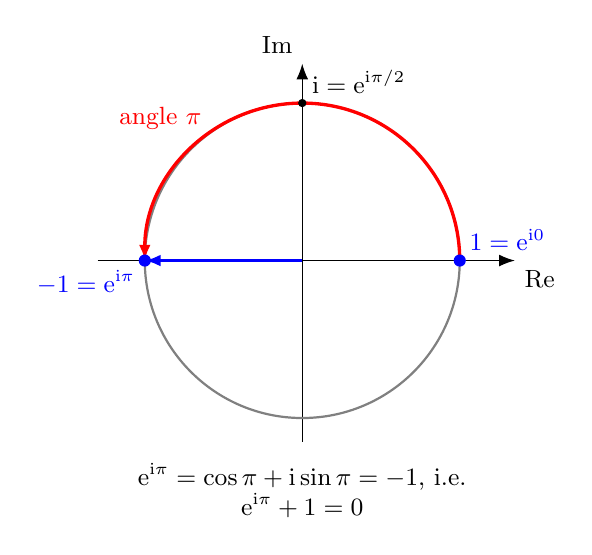
\begin{tikzpicture}[every node/.style={font=\small}, >={Latex[length=2mm]}]
	\draw[->] (-2.6,0) -- (2.7,0) node[below right] {$\mathrm{Re}$};
	\draw[->] (0,-2.3) -- (0,2.5) node[above left] {$\mathrm{Im}$};
	\draw[gray, thick] (0,0) circle (2);
	\draw[red, very thick, ->] (2,0) arc (0:180:2);
	\node[red] at (135:2.55) {angle $\pi$};
	\fill[blue] (2,0) circle (2.2pt) node[above right] {$1=\mathrm{e}^{\mathrm{i}0}$};
	\fill[blue] (-2,0) circle (2.2pt) node[below left] {$-1=\mathrm{e}^{\mathrm{i}\pi}$};
	\fill (0,2) circle (1.5pt) node[above right] {$\mathrm{i}=\mathrm{e}^{\mathrm{i}\pi/2}$};
	\draw[->, blue, very thick] (0,0) -- (-2,0);
	\node[anchor=north, align=center] at (0,-2.45) {$\mathrm{e}^{\mathrm{i}\pi}=\cos\pi+\mathrm{i}\sin\pi=-1$, i.e.\\ $\mathrm{e}^{\mathrm{i}\pi}+1=0$};
\end{tikzpicture}
\end{document}
